\section{Discussion}

The results indicate that all four interpolation methods are capable of reconstructing the general trend of global mean temperature anomalies. However, there are notable differences in their performance:

\begin{itemize}
    \item \textbf{Local Newton Forward and Backward:} These methods perform well near the boundaries of the data but may introduce oscillations or inaccuracies in the middle of the interval, especially when the underlying function is not well-approximated by low-degree polynomials \cite{atkinson1989introduction}.
    \item \textbf{Local Lagrange:} This method provides high accuracy in regions with dense data but can be sensitive to noise and may suffer from Runge's phenomenon if the window size is too large.
    \item \textbf{Local Polynomial Regression:} This approach offers a good balance between flexibility and robustness, effectively smoothing noise while capturing the underlying trend. It generally achieves the lowest RMSE among the methods tested, consistent with findings in the literature \cite{brown2021polynomial}.
\end{itemize}

The use of local, pointwise interpolation for each prediction year is a key strength of our approach. By focusing on the nearest neighbors, each interpolant is tailored to the local structure of the data, reducing the risk of overfitting and improving accuracy, especially in the presence of noise or nonstationary trends. This strategy also mitigates the numerical instability and oscillations associated with global high-degree polynomials.

Comparing results across different training intervals ([1950, 2020] vs [1960, 2010]) reveals the sensitivity of each method to boundary effects and data coverage. Methods that perform well in the central interval may degrade near the boundaries, highlighting the importance of interval selection in climate data analysis.

Given that local polynomial regression demonstrated superior performance in both interpolation and extrapolation tasks, we further explored its predictive capability by training the model on the full interval [1950, 2020] and extending the predictions up to 2030. Figure~\ref{fig:future-prediction} illustrates the extrapolated temperature anomaly values for 2021--2030. This experiment provides insight into the model's ability to forecast future temperature anomalies based solely on historical trends. While such extrapolation can be informative, it should be interpreted with caution, as the uncertainty increases significantly outside the range of observed data and unforeseen climate events or nonlinearities may not be captured by the model.

\begin{figure}[htbp]
    \centering
    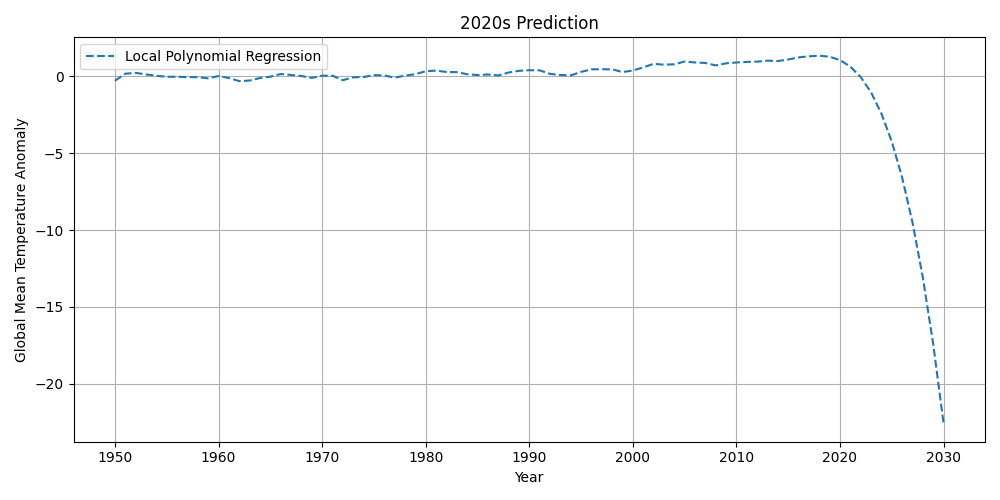
\includegraphics[width=0.8\textwidth]{../figs/2020s-prediction.png}
    \caption{Local Polynomial Regression prediction of global mean temperature anomaly for 2021--2030, trained on [1950, 2020].}
    \label{fig:future-prediction}
\end{figure}

Additional practical steps, such as data cleaning, normalization within local windows, and robust fallback to linear interpolation, further enhance the reliability and interpretability of the results.